% Options for packages loaded elsewhere
\PassOptionsToPackage{unicode}{hyperref}
\PassOptionsToPackage{hyphens}{url}
%
\documentclass[
]{article}
\usepackage{amsmath,amssymb}
\usepackage{iftex}
\ifPDFTeX
  \usepackage[T1]{fontenc}
  \usepackage[utf8]{inputenc}
  \usepackage{textcomp} % provide euro and other symbols
\else % if luatex or xetex
  \usepackage{unicode-math} % this also loads fontspec
  \defaultfontfeatures{Scale=MatchLowercase}
  \defaultfontfeatures[\rmfamily]{Ligatures=TeX,Scale=1}
\fi
\usepackage{lmodern}
\ifPDFTeX\else
  % xetex/luatex font selection
\fi
% Use upquote if available, for straight quotes in verbatim environments
\IfFileExists{upquote.sty}{\usepackage{upquote}}{}
\IfFileExists{microtype.sty}{% use microtype if available
  \usepackage[]{microtype}
  \UseMicrotypeSet[protrusion]{basicmath} % disable protrusion for tt fonts
}{}
\makeatletter
\@ifundefined{KOMAClassName}{% if non-KOMA class
  \IfFileExists{parskip.sty}{%
    \usepackage{parskip}
  }{% else
    \setlength{\parindent}{0pt}
    \setlength{\parskip}{6pt plus 2pt minus 1pt}}
}{% if KOMA class
  \KOMAoptions{parskip=half}}
\makeatother
\usepackage{xcolor}
\usepackage[margin=1in]{geometry}
\usepackage{color}
\usepackage{fancyvrb}
\newcommand{\VerbBar}{|}
\newcommand{\VERB}{\Verb[commandchars=\\\{\}]}
\DefineVerbatimEnvironment{Highlighting}{Verbatim}{commandchars=\\\{\}}
% Add ',fontsize=\small' for more characters per line
\usepackage{framed}
\definecolor{shadecolor}{RGB}{248,248,248}
\newenvironment{Shaded}{\begin{snugshade}}{\end{snugshade}}
\newcommand{\AlertTok}[1]{\textcolor[rgb]{0.94,0.16,0.16}{#1}}
\newcommand{\AnnotationTok}[1]{\textcolor[rgb]{0.56,0.35,0.01}{\textbf{\textit{#1}}}}
\newcommand{\AttributeTok}[1]{\textcolor[rgb]{0.13,0.29,0.53}{#1}}
\newcommand{\BaseNTok}[1]{\textcolor[rgb]{0.00,0.00,0.81}{#1}}
\newcommand{\BuiltInTok}[1]{#1}
\newcommand{\CharTok}[1]{\textcolor[rgb]{0.31,0.60,0.02}{#1}}
\newcommand{\CommentTok}[1]{\textcolor[rgb]{0.56,0.35,0.01}{\textit{#1}}}
\newcommand{\CommentVarTok}[1]{\textcolor[rgb]{0.56,0.35,0.01}{\textbf{\textit{#1}}}}
\newcommand{\ConstantTok}[1]{\textcolor[rgb]{0.56,0.35,0.01}{#1}}
\newcommand{\ControlFlowTok}[1]{\textcolor[rgb]{0.13,0.29,0.53}{\textbf{#1}}}
\newcommand{\DataTypeTok}[1]{\textcolor[rgb]{0.13,0.29,0.53}{#1}}
\newcommand{\DecValTok}[1]{\textcolor[rgb]{0.00,0.00,0.81}{#1}}
\newcommand{\DocumentationTok}[1]{\textcolor[rgb]{0.56,0.35,0.01}{\textbf{\textit{#1}}}}
\newcommand{\ErrorTok}[1]{\textcolor[rgb]{0.64,0.00,0.00}{\textbf{#1}}}
\newcommand{\ExtensionTok}[1]{#1}
\newcommand{\FloatTok}[1]{\textcolor[rgb]{0.00,0.00,0.81}{#1}}
\newcommand{\FunctionTok}[1]{\textcolor[rgb]{0.13,0.29,0.53}{\textbf{#1}}}
\newcommand{\ImportTok}[1]{#1}
\newcommand{\InformationTok}[1]{\textcolor[rgb]{0.56,0.35,0.01}{\textbf{\textit{#1}}}}
\newcommand{\KeywordTok}[1]{\textcolor[rgb]{0.13,0.29,0.53}{\textbf{#1}}}
\newcommand{\NormalTok}[1]{#1}
\newcommand{\OperatorTok}[1]{\textcolor[rgb]{0.81,0.36,0.00}{\textbf{#1}}}
\newcommand{\OtherTok}[1]{\textcolor[rgb]{0.56,0.35,0.01}{#1}}
\newcommand{\PreprocessorTok}[1]{\textcolor[rgb]{0.56,0.35,0.01}{\textit{#1}}}
\newcommand{\RegionMarkerTok}[1]{#1}
\newcommand{\SpecialCharTok}[1]{\textcolor[rgb]{0.81,0.36,0.00}{\textbf{#1}}}
\newcommand{\SpecialStringTok}[1]{\textcolor[rgb]{0.31,0.60,0.02}{#1}}
\newcommand{\StringTok}[1]{\textcolor[rgb]{0.31,0.60,0.02}{#1}}
\newcommand{\VariableTok}[1]{\textcolor[rgb]{0.00,0.00,0.00}{#1}}
\newcommand{\VerbatimStringTok}[1]{\textcolor[rgb]{0.31,0.60,0.02}{#1}}
\newcommand{\WarningTok}[1]{\textcolor[rgb]{0.56,0.35,0.01}{\textbf{\textit{#1}}}}
\usepackage{longtable,booktabs,array}
\usepackage{calc} % for calculating minipage widths
% Correct order of tables after \paragraph or \subparagraph
\usepackage{etoolbox}
\makeatletter
\patchcmd\longtable{\par}{\if@noskipsec\mbox{}\fi\par}{}{}
\makeatother
% Allow footnotes in longtable head/foot
\IfFileExists{footnotehyper.sty}{\usepackage{footnotehyper}}{\usepackage{footnote}}
\makesavenoteenv{longtable}
\usepackage{graphicx}
\makeatletter
\def\maxwidth{\ifdim\Gin@nat@width>\linewidth\linewidth\else\Gin@nat@width\fi}
\def\maxheight{\ifdim\Gin@nat@height>\textheight\textheight\else\Gin@nat@height\fi}
\makeatother
% Scale images if necessary, so that they will not overflow the page
% margins by default, and it is still possible to overwrite the defaults
% using explicit options in \includegraphics[width, height, ...]{}
\setkeys{Gin}{width=\maxwidth,height=\maxheight,keepaspectratio}
% Set default figure placement to htbp
\makeatletter
\def\fps@figure{htbp}
\makeatother
\setlength{\emergencystretch}{3em} % prevent overfull lines
\providecommand{\tightlist}{%
  \setlength{\itemsep}{0pt}\setlength{\parskip}{0pt}}
\setcounter{secnumdepth}{5}
\ifLuaTeX
  \usepackage{selnolig}  % disable illegal ligatures
\fi
\usepackage{bookmark}
\IfFileExists{xurl.sty}{\usepackage{xurl}}{} % add URL line breaks if available
\urlstyle{same}
\hypersetup{
  hidelinks,
  pdfcreator={LaTeX via pandoc}}

\author{}
\date{\vspace{-2.5em}}

\begin{document}

{
\setcounter{tocdepth}{2}
\tableofcontents
}
\section*{Presentación}\label{presentaciuxf3n}
\addcontentsline{toc}{section}{Presentación}

\subsection*{Objetivo}\label{objetivo}
\addcontentsline{toc}{subsection}{Objetivo}

El objetivo de estos ejercicios es proporcionar unos materiales de soporte para la asignatura de ``Inferencia Estadística'' del \href{https://www.uoc.edu/es/estudios/masters/master-universitario-bioinformatica-bioestadistica}{Máster interuniversitario de Bioiestadística y Bioinformática} impartido conjuntamente por la \href{https://www.uoc.edu}{Universitat Oberta de Catalunya (UOC)} y la \href{https://www.ub.edu}{Universidad de Barcelona (UB)}.

Esta asignatura adolece de las características habituales de las asignaturas de posgrado, y especialmente de un posgrado de estadística (y bioinformática), que muestran algunas de las cosas que no debe de ser esta asignatura:

Tal como se indica en la introducción a las notas de soporte del curso, este debería:

\begin{itemize}
\tightlist
\item
  Servir para repasar y consolidar los conceptos básicos que la mayoría de estudiantes traerán consigo.
\item
  Además, y sobretodo, debe proporcionar una visión general, lo más completa posible dentro de las limitaciones de tiempo, del campo de la inferencia estadística
\end{itemize}

Y, naturalmente, una de las formas de consolidar conocimientos, como en cualquier disciplina cuantitatva,es a traves de la resolución de ejercicios que permiten reflexionar, comprender y ver como se aplican los conceptos teóricos introducidos.

Para ello, estos materiales contienen una serie de ejercicios similares a los que se proponen en las actividades y pruebas de evaluación continua de la asignatura.

La mayoría de los ejercicios estan resueltos, pero \emph{es importante intentar resolverlos de forma autónoma antes de consultar la solución}.

En general los ejercicios no presuponen ningún conocimiento especial de matemáticas, más allá de las habilidades básicas que se adquieren durante los estudios de una carrera de ciencias o de ingeniería.

\section{Probabilidad y Experimentos aleatorios}\label{probabilidad-y-experimentos-aleatorios}

\subsection{Problema 1}\label{problema-1}

Sean \(A\) y \(B\) dos sucesos. Suponiendo que \(P(A)=0.3, P(B)=0.6\), y \(P(A \cap B)=0.1\), calcula las siguientes probabilidades:

\begin{enumerate}
\def\labelenumi{\alph{enumi})}
\item
  \(P(A \cup B)\)
\item
  \(P(A^c)\)
\item
  \(P(A c \cap B)\)
\item
  \(P(A \cap B^c)\)
\item
  \(P(A^c \cap B^c)\)
\end{enumerate}

\subsubsection{Solución}\label{soluciuxf3n}

\begin{enumerate}
\def\labelenumi{\alph{enumi}.}
\tightlist
\item
  \(P(A \cup B)=P(A)+P(B)-P(A \cap B)=0.3+0.6-0.1=0.8\)
\item
  \(P\left(A^{c}\right)=1-P(A)=1-0.3=0.7\)
\item
  \(P\left(A^{c} \cap B\right)=P(B)-P(A \cap B)=0.6-0.1=0.5\)
\item
  \(P\left(A \cap B^{c}\right)=P(A)-P(A \cap B)=0.3-0.1=0.2\)
\item
  \(P\left(A^{c} \cap B^{c}\right)=1-P(A \cup B)=1-0.8=0.2\)
\end{enumerate}

\subsection{Problema 2}\label{problema-2}

Una población está afectada por tres enfermedades diferentes A, B i C. La probabilidad de que una persona sufra \(A\) es 0.30 , la probabilidad de que sufra \(B\) es 0.20 y la probabilidad de que sufra \(C\) es 0.15 . La probabilidad de que una persona sufra \(A\) y \(B\) es 0.12 , la que sufra \(A\) y \(C\) es 0.09 y la que sufra \(B\) y \(C\) es 0.06 . La probabilidad de que una persona sufra las tres enfermedades es 0.03 . Se piden las probabilidades de que una persona escogida al azar:

\begin{enumerate}

\item padezca al menos una enfermedad

\item sólo sufra $A$

\item sufra B o C, pero no sufra A

\item sufra A o no sufra ni B ni C.

\end{enumerate}

\subsubsection{Solución}\label{soluciuxf3n-1}

\begin{center}\rule{0.5\linewidth}{0.5pt}\end{center}

\begin{enumerate}
\def\labelenumi{\alph{enumi})}
\tightlist
\item
  \textbf{¿Cuál es la probabilidad de que una persona padezca al menos una enfermedad?}
\end{enumerate}

Queremos calcular la probabilidad de que una persona sufra al menos una de las tres enfermedades, es decir, \(P(A \cup B \cup C)\).

Para calcular \(P(A \cup B \cup C)\), usamos la regla de inclusión-exclusión:

\[
P(A \cup B \cup C) = P(A) + P(B) + P(C) - P(A \cap B) - P(A \cap C) - P(B \cap C) + P(A \cap B \cap C)
\]

Sustituyendo los valores dados en el enunciado:

\[
P(A \cup B \cup C) = 0.30 + 0.20 + 0.15 - 0.12 - 0.09 - 0.06 + 0.03 = 0.41
\]

Por lo tanto, la probabilidad de que una persona padezca al menos una enfermedad es \textbf{0.41}.

\begin{center}\rule{0.5\linewidth}{0.5pt}\end{center}

\begin{enumerate}
\def\labelenumi{\alph{enumi})}
\setcounter{enumi}{1}
\tightlist
\item
  \textbf{¿Cuál es la probabilidad de que una persona solo sufra \(A\)?}
\end{enumerate}

Para resolver esto, necesitamos calcular la probabilidad de que la persona sufra \(A\), pero no \(B\) ni \(C\), es decir, \(P(A \cap B^c \cap C^c)\).

Podemos calcular \(P(A \cap B^c \cap C^c)\) restando de \(P(A)\) la probabilidad de que la persona sufra \(A\) junto con alguna de las otras dos enfermedades:

\[
P(A \cap B^c \cap C^c) = P(A) - P(A \cap B) - P(A \cap C) + P(A \cap B \cap C)
\]

Sustituyendo los valores:

\[
P(A \cap B^c \cap C^c) = 0.30 - 0.12 - 0.09 + 0.03 = 0.12
\]

Por lo tanto, la probabilidad de que una persona solo sufra \(A\) es \textbf{0.12}.

\begin{center}\rule{0.5\linewidth}{0.5pt}\end{center}

\begin{enumerate}
\def\labelenumi{\alph{enumi})}
\setcounter{enumi}{2}
\tightlist
\item
  \textbf{¿Cuál es la probabilidad de que una persona sufra \(B\) o \(C\), pero no sufra \(A\)?}
\end{enumerate}

Aquí buscamos la probabilidad \(P(A^c \cap (B \cup C))\), es decir, la probabilidad de que la persona no tenga \(A\), pero tenga \(B\) o \(C\).

Primero, calculamos \(P(B \cup C)\) utilizando la regla de inclusión-exclusión:

\[
P(B \cup C) = P(B) + P(C) - P(B \cap C)
\]

Sustituyendo los valores:

\[
P(B \cup C) = 0.20 + 0.15 - 0.06 = 0.29
\]

Ahora, para calcular \(P(A^c \cap (B \cup C))\), restamos de \(P(B \cup C)\) la probabilidad de que la persona tenga \(A\) y alguna de las enfermedades \(B\) o \(C\), es decir, \(P(A \cap (B \cup C))\):

\[
P(A \cap (B \cup C)) = P(A \cap B) + P(A \cap C) - P(A \cap B \cap C)
\]

Sustituyendo los valores:

\[
P(A \cap (B \cup C)) = 0.12 + 0.09 - 0.03 = 0.18
\]

Finalmente, restamos:

\[
P(A^c \cap (B \cup C)) = P(B \cup C) - P(A \cap (B \cup C)) = 0.29 - 0.18 = 0.11
\]

Por lo tanto, la probabilidad de que una persona sufra \(B\) o \(C\), pero no \(A\), es \textbf{0.11}.

\begin{center}\rule{0.5\linewidth}{0.5pt}\end{center}

\begin{enumerate}
\def\labelenumi{\alph{enumi})}
\setcounter{enumi}{3}
\tightlist
\item
  \textbf{¿Cuál es la probabilidad de que una persona sufra \(A\) o no sufra ni \(B\) ni \(C\)?}
\end{enumerate}

Aquí buscamos la probabilidad \(P(A \cup (B^c \cap C^c))\), es decir, que la persona sufra \(A\) o que no sufra ni \(B\) ni \(C\).

Primero, calculamos \(P(B^c \cap C^c)\), que es la probabilidad de que la persona no sufra ni \(B\) ni \(C\). Esto es simplemente \(1 - P(B \cup C)\), que ya calculamos previamente:

\[
P(B^c \cap C^c) = 1 - P(B \cup C) = 1 - 0.29 = 0.71
\]

Ahora, aplicamos la regla de la unión para calcular \(P(A \cup (B^c \cap C^c))\):

\[
P(A \cup (B^c \cap C^c)) = P(A) + P(B^c \cap C^c) - P(A \cap B^c \cap C^c)
\]

Ya calculamos \(P(B^c \cap C^c)\), y sabemos que \(P(A \cap B^c \cap C^c)\) es la probabilidad de que una persona solo sufra \(A\), que también calculamos previamente:

\[
P(A \cap B^c \cap C^c) = 0.12
\]

Sustituyendo los valores:

\[
P(A \cup (B^c \cap C^c)) = 0.30 + 0.71 - 0.12 = 0.89
\]

Por lo tanto, la probabilidad de que una persona sufra \(A\) o no sufra ni \(B\) ni \(C\) es \textbf{0.89}.

\textbf{Resumiendo:}

\begin{enumerate}
\def\labelenumi{\arabic{enumi}.}
\tightlist
\item
  La probabilidad de que una persona padezca al menos una enfermedad es \textbf{0.41}.
\item
  La probabilidad de que una persona solo sufra \(A\) es \textbf{0.12}.
\item
  La probabilidad de que una persona sufra \(B\) o \(C\), pero no \(A\), es \textbf{0.11}.
\item
  La probabilidad de que una persona sufra \(A\) o no sufra ni \(B\) ni \(C\) es \textbf{0.89}.
\end{enumerate}

\subsection{Problema 3}\label{problema-3}

Por los síntomas observados en un enfermo, y según la experiencia acumulada en un gran número de situaciones similares, se deduce que ha podido coger la enfermedad \(A\) con probabilidad \(1 / 3\), o la enfermedad \(B\) con probabilidad \(2 / 3\). Con el fin de precisar el diagnóstico, se hace un análisis clínico al enfermo con dos resultados posibles, positivo o negativo. Se sabe, también por experiencia, que en los pacientes que tienen la enfermedad En el análisis es positiva con probabilidad 0.99 , y en los que padecen la enfermedad B lo es con probabilidad 0.06

\begin{enumerate}
\def\labelenumi{\alph{enumi})}
\item
  ¿Cuál es la probabilidad de que el análisis dé un
  resultado negativo?
\item
  Si el resultado ha sido positivo, ¿cuál es la probabilidad de que el paciente sufra la enfermedad A? ¿Y la probabilidad de que padezca la enfermedad B?
\end{enumerate}

\subsubsection{Solución}\label{soluciuxf3n-2}

\begin{enumerate}
\def\labelenumi{\alph{enumi}.}
\item
  \[
  \begin{aligned}
  P(Neg)&=P(Neg|A) \cdot  P(A)+P(Neg|B) \cdot  P(B)=
  \\&= 0.01 \cdot 1 / 3+0.94 \cdot 2 / 3=0.63
  \end{aligned}
  \]
\item
\end{enumerate}

\[
\begin{aligned}
\mathrm{P}(\mathrm{A} | Pos )&=\frac{P(\text { Pos } | A) P(A)}{P(\text { Pos})}=0.8919, \quad \text{para A},\\
\mathrm{P}(\mathrm{B} | Pos)&=1-\mathrm{P}(\mathrm{A} / Positiu )=0.1081, \quad \text{para $B$}.
\end{aligned}
\]

Las probabilidades las hemos calculado con R a partir de la información del enunciado:

\begin{Shaded}
\begin{Highlighting}[]
\NormalTok{pA}\OtherTok{\textless{}{-}}\DecValTok{1}\SpecialCharTok{/}\DecValTok{3}
\NormalTok{pB}\OtherTok{\textless{}{-}}\DecValTok{2}\SpecialCharTok{/}\DecValTok{3}
\NormalTok{ppA}\OtherTok{\textless{}{-}}\FloatTok{0.99}
\NormalTok{ppB}\OtherTok{\textless{}{-}}\FloatTok{0.06}
\NormalTok{pn}\OtherTok{\textless{}{-}}\NormalTok{(}\DecValTok{1}\SpecialCharTok{{-}}\NormalTok{ppA)}\SpecialCharTok{*}\NormalTok{pA}\SpecialCharTok{+}\NormalTok{(}\DecValTok{1}\SpecialCharTok{{-}}\NormalTok{ppB)}\SpecialCharTok{*}\NormalTok{pB}
\NormalTok{pn}
\end{Highlighting}
\end{Shaded}

\begin{verbatim}
## [1] 0.63
\end{verbatim}

\subsection{Problema 4}\label{problema-4}

El embolismo pulmonar es una condición relativamente común que necesita hospitalización y que a menudo ocurre en pacientes hospitalizados. La presión arterial menor de 90 mm HG es uno de los criterios importantes para diagnosticar esta condición. Supongamos que la sensibilidad del test es del 95\% y la especificidad del test es del 75\% y la prevalencia es del 20\%.

\begin{enumerate}
\def\labelenumi{\alph{enumi})}
\item
  Calcula el valor predictivo positivo del test.
\item
  Calcula el valor predictivo negativo del test.
\item
  Responde a las preguntas anteriores si la prevalencia fuera del \(80 \%\).
\end{enumerate}

\subsubsection{Solución}\label{soluciuxf3n-3}

\begin{enumerate}
\def\labelenumi{\alph{enumi})}
\tightlist
\item
  Calcula el valor predictivo positivo del test
\end{enumerate}

\[
V P+=P(\text { Embolismo } / \text { Test }+)=\frac{\text { Sens}\times\text{Prev }}{\text { Sens}\times\text{Prev }+(1-\text { Esp })(1-\text { Prev })}
\]

\begin{Shaded}
\begin{Highlighting}[]
\NormalTok{sens}\OtherTok{\textless{}{-}}\FloatTok{0.95}
\NormalTok{esp}\OtherTok{\textless{}{-}}\FloatTok{0.75}
\NormalTok{prev}\OtherTok{\textless{}{-}}\FloatTok{0.20}
\NormalTok{vpp}\OtherTok{\textless{}{-}}\NormalTok{(sens}\SpecialCharTok{*}\NormalTok{prev)}\SpecialCharTok{/}\NormalTok{(sens}\SpecialCharTok{*}\NormalTok{prev}\SpecialCharTok{+}\NormalTok{(}\DecValTok{1}\SpecialCharTok{{-}}\NormalTok{esp)}\SpecialCharTok{*}\NormalTok{(}\DecValTok{1}\SpecialCharTok{{-}}\NormalTok{prev))}
\NormalTok{vpp}
\end{Highlighting}
\end{Shaded}

\begin{verbatim}
## [1] 0.4871795
\end{verbatim}

\begin{enumerate}
\def\labelenumi{\alph{enumi})}
\setcounter{enumi}{1}
\tightlist
\item
  Calcula el valor predictivo negativo del test
\end{enumerate}

\[
V P-=\frac{\operatorname{Esp}(1-\operatorname{Prev})}{\operatorname{Esp}(1-\operatorname{Prev})+(1-\text { Sens }) \operatorname{Prev}}
\]

\begin{Shaded}
\begin{Highlighting}[]
\NormalTok{vpn}\OtherTok{\textless{}{-}}\NormalTok{(esp}\SpecialCharTok{*}\NormalTok{(}\DecValTok{1}\SpecialCharTok{{-}}\NormalTok{prev))}\SpecialCharTok{/}\NormalTok{(esp}\SpecialCharTok{*}\NormalTok{(}\DecValTok{1}\SpecialCharTok{{-}}\NormalTok{prev)}\SpecialCharTok{+}\NormalTok{(}\DecValTok{1}\SpecialCharTok{{-}}\NormalTok{sens)}\SpecialCharTok{*}\NormalTok{prev)}
\NormalTok{vpn}
\end{Highlighting}
\end{Shaded}

\begin{verbatim}
## [1] 0.9836066
\end{verbatim}

Como se observa al tratarse de una prueba muy sensible y poco específica hay pocos falsos negativos y cuando el test da negativo hay una probabilidad muy alta (0.98) de que el individuo sea sano. No así cuando da positivo. Sólo el \(48 \%\) serán verdaderos enfermos.

\begin{enumerate}
\def\labelenumi{\alph{enumi})}
\setcounter{enumi}{2}
\tightlist
\item
  Responde a las preguntas anteriores si la prevalencia fuera del 80\%
\end{enumerate}

\begin{Shaded}
\begin{Highlighting}[]
\NormalTok{prev}\OtherTok{\textless{}{-}}\FloatTok{0.80}
\NormalTok{vpp}\OtherTok{\textless{}{-}}\NormalTok{(sens}\SpecialCharTok{*}\NormalTok{prev)}\SpecialCharTok{/}\NormalTok{(sens}\SpecialCharTok{*}\NormalTok{prev}\SpecialCharTok{+}\NormalTok{(}\DecValTok{1}\SpecialCharTok{{-}}\NormalTok{esp)}\SpecialCharTok{*}\NormalTok{(}\DecValTok{1}\SpecialCharTok{{-}}\NormalTok{prev))}
\NormalTok{vpp}
\end{Highlighting}
\end{Shaded}

\begin{verbatim}
## [1] 0.9382716
\end{verbatim}

\begin{Shaded}
\begin{Highlighting}[]
\NormalTok{vpn}\OtherTok{\textless{}{-}}\NormalTok{(esp}\SpecialCharTok{*}\NormalTok{(}\DecValTok{1}\SpecialCharTok{{-}}\NormalTok{prev))}\SpecialCharTok{/}\NormalTok{(esp}\SpecialCharTok{*}\NormalTok{(}\DecValTok{1}\SpecialCharTok{{-}}\NormalTok{prev)}\SpecialCharTok{+}\NormalTok{(}\DecValTok{1}\SpecialCharTok{{-}}\NormalTok{sens)}\SpecialCharTok{*}\NormalTok{prev)}
\NormalTok{vpn}
\end{Highlighting}
\end{Shaded}

\begin{verbatim}
## [1] 0.7894737
\end{verbatim}

Si la prevalencia es más alta, el VP- sigue siendo alto, aunque no tanto pero hemos aumentado el VP+ hasta el 93\% y no habrá tantos falsos positivos. Lo que está claro es el VPN y el VPP dependen de la prevalencia de la enfermedad.

\subsection{Problema 5}\label{problema-5}

Un índice que evalúa el síndrome de la muerte súbita (SMS) tiene una sensibilidad del \(68 \%\) y una especificidad del \(82 \%\). ¿Cuáles son los valores predictivos positivo y negativo del índice si se aplica a una población donde se producen un \(0,21 \%\) de muertes súbitas sobre el total de nacimientos?

\subsubsection{Solución}\label{soluciuxf3n-4}

La prevalencia del síndrome de la muerte súbita en la población es del 0.21\%, es decir 0.0021.

Nos piden que calculemos respectivamente los valores predictivos positivo y negativo del test. Es decir, que tan bien funciona el test para detectar la enfermedad (\(SMS\)) cuando da un resultado positivo (\(T+\)) y para indicar su ausencia (\(SMS^c\)), mediante un resultado negativo (\(T-\)).

\[
VP+ = P[SMS | T+],\qquad VP- = P[SMS^c | T-],
\]

Puede hacerse el cálculo directamente a partir de las probabilidades condicionadas.

\[
\begin{aligned}
VP+ & = P[SMS | T+]= \frac {P[T+ | SMS]\times P[SMS]}{P[T+]} =\\
& = \frac {P[T+ | SMS]\times P[SMS]}
{P[T+|SMS]\times P[SMS]+ P[T+|SMS^c]\times P[SMS^c]}=\\
& = \frac{\text {Sensibilidad}\times \text{Prevalencia}}
{\text {Sensibilidad}\times \text{Prevalencia}+
\text {1-Especificidad}\times \text{1-Prevalencia}}
\end{aligned}
\]

De forma análoga:

\[
\begin{aligned}
VP- & = P[SMS^c | T-]= \frac {P[T- | SMS^c]\times P[SMS^c]}{P[T-]} =\\
& = \frac {P[T- | SMS^c]\times P[SMS^c]}{P[T- | SMS^c]\times P[SMS^c] + P[T- | SMS]\times P[SMS]}=\\
& = \frac{\text {Especificidad}\times \text{1-Prevalencia}}
{\text {Especificidad}\times \text{1-Prevalencia}+
\text {1-Sensibilidad}\times \text{Prevalencia}}
\end{aligned}
\]

Estos cálculos se reañlizan de forma imediata usando R:

\begin{Shaded}
\begin{Highlighting}[]
\NormalTok{sensi }\OtherTok{\textless{}{-}} \FloatTok{0.68}
\NormalTok{espec }\OtherTok{\textless{}{-}} \FloatTok{0.82}
\NormalTok{prev }\OtherTok{\textless{}{-}} \FloatTok{0.0021}
\NormalTok{vp.pos }\OtherTok{\textless{}{-}}\NormalTok{ (sensi }\SpecialCharTok{*}\NormalTok{ prev )}\SpecialCharTok{/}\NormalTok{ (sensi }\SpecialCharTok{*}\NormalTok{ prev }\SpecialCharTok{+}\NormalTok{ (}\DecValTok{1}\SpecialCharTok{{-}}\NormalTok{espec)}\SpecialCharTok{*}\NormalTok{ (}\DecValTok{1}\SpecialCharTok{{-}}\NormalTok{prev))}
\FunctionTok{cat}\NormalTok{ (}\StringTok{"El valor predictivo positivo es: "}\NormalTok{, vp.pos)}
\end{Highlighting}
\end{Shaded}

\begin{verbatim}
## El valor predictivo positivo es:  0.007887324
\end{verbatim}

\begin{Shaded}
\begin{Highlighting}[]
\NormalTok{vp.neg }\OtherTok{\textless{}{-}}\NormalTok{ (espec }\SpecialCharTok{*}\NormalTok{ (}\DecValTok{1}\SpecialCharTok{{-}}\NormalTok{prev) )}\SpecialCharTok{/}\NormalTok{ (espec }\SpecialCharTok{*}\NormalTok{ (}\DecValTok{1}\SpecialCharTok{{-}}\NormalTok{prev) }\SpecialCharTok{+}\NormalTok{ (}\DecValTok{1}\SpecialCharTok{{-}}\NormalTok{sensi)}\SpecialCharTok{*}\NormalTok{ (prev))}
\FunctionTok{cat}\NormalTok{ (}\StringTok{"El valor predictivo negativo es: "}\NormalTok{, vp.neg)}
\end{Highlighting}
\end{Shaded}

\begin{verbatim}
## El valor predictivo negativo es:  0.9991794
\end{verbatim}

Como en el caso anterior, podemos ver que. al ser la prevalencia muy baja, el valor predicpositivo del test también lo es puesto que un test + tan solo indica en un 0,79\% de veces la presencia del síndrome, correctamente.

\section{Variables aleatorias y Distribuciones de probabilidad}\label{variables-aleatorias-y-distribuciones-de-probabilidad}

\subsection{Ejercicio 2.1}\label{ejercicio-2.1}

Se sabe que la presencia de algunas mutaciones en una región genómica puede influir en la sobreexpresión (``Up'') o la inhibición (``Down'') de dos genes distintos. Se conocen 6 variantes de dicha mutación y, dado que los efectos de la sobreexpresión de los dos genes son muy similares se ha optado por contar únicamente cuántos genes se sobre-expresan en presencia de cada una de ellas (un individuo puede presentar una única variante). Un estudio realizado sobre 300 pacientes ha permitido estimar las siguientes probabilidades de aparición de cada mutación así como el número de genes sobre-expresados asociados a las mismas. Los resultados se encuentran disponibles en la tabla siguiente:

\begin{longtable}[]{@{}ccc@{}}
\toprule\noalign{}
Mutación & Probabilidad & \(N^{\circ}\) de genes \\
\midrule\noalign{}
\endhead
\bottomrule\noalign{}
\endlastfoot
\(e_{1}\) & 0.15 & 0 \\
\(e_{2}\) & 0.13 & 1 \\
\(e_{3}\) & 0.07 & 1 \\
\(e_{4}\) & 0.30 & 2 \\
\(e_{5}\) & 0.20 & 2 \\
\(e_{6}\) & 0.15 & 0 \\
\end{longtable}

Consideremos la variable aleatoria: \(X=\) ``Número de genes sobre expresados''

\begin{enumerate}
\def\labelenumi{\arabic{enumi}.}
\item
  Obtener su distribución de probabilidad y representarla gráficamente
\item
  Calcular la esperanza y la varianza de dicha variable
\end{enumerate}

\textbf{SOLUCIÓN}

La variable aleatoria que nos interesa es \(X=\) ``Número de genes sobre-expresados''.

\subsubsection{Distribución de probabilidad}\label{distribuciuxf3n-de-probabilidad}

Para obtener la distribución de probabilidad de \(X\), necesitamos sumar las probabilidades de las mutaciones que tienen el mismo número de genes sobre-expresados.

Los posibles valores de \(X\) son 0, 1 y 2. A continuación calculamos la probabilidad de cada uno:

\begin{itemize}
\tightlist
\item
  Para \(X = 0\), las mutaciones son \(e_1\) y \(e_6\):
\end{itemize}

\[
P(X = 0) = P(e_1) + P(e_6) = 0.15 + 0.15 = 0.30
\]

\begin{itemize}
\tightlist
\item
  Para \(X = 1\), las mutaciones son \(e_2\) y \(e_3\):
\end{itemize}

\[
P(X = 1) = P(e_2) + P(e_3) = 0.13 + 0.07 = 0.20
\]

\begin{itemize}
\tightlist
\item
  Para \(X = 2\), las mutaciones son \(e_4\) y \(e_5\):
\end{itemize}

\[
P(X = 2) = P(e_4) + P(e_5) = 0.30 + 0.20 = 0.50
\]

La distribución de probabilidad de \(X\) es la siguiente:

\[
P(X = x) =
\begin{cases}
0.30 & \text{si } x = 0, \\
0.20 & \text{si } x = 1, \\
0.50 & \text{si } x = 2.
\end{cases}
\]

Podemos representarla gráficamente usando R:

\begin{Shaded}
\begin{Highlighting}[]
\CommentTok{\# Valores de X y sus probabilidades}
\NormalTok{X\_values }\OtherTok{\textless{}{-}} \FunctionTok{c}\NormalTok{(}\DecValTok{0}\NormalTok{, }\DecValTok{1}\NormalTok{, }\DecValTok{2}\NormalTok{)}
\NormalTok{probabilities }\OtherTok{\textless{}{-}} \FunctionTok{c}\NormalTok{(}\FloatTok{0.30}\NormalTok{, }\FloatTok{0.20}\NormalTok{, }\FloatTok{0.50}\NormalTok{)}

\CommentTok{\# Crear el gráfico}
\FunctionTok{barplot}\NormalTok{(probabilities, }\AttributeTok{names.arg =}\NormalTok{ X\_values, }\AttributeTok{col =} \StringTok{"lightblue"}\NormalTok{,}
        \AttributeTok{main =} \StringTok{"Distribución de Probabilidad de X"}\NormalTok{,}
        \AttributeTok{xlab =} \StringTok{"Número de genes sobre{-}expresados"}\NormalTok{, }\AttributeTok{ylab =} \StringTok{"Probabilidad"}\NormalTok{)}
\end{Highlighting}
\end{Shaded}

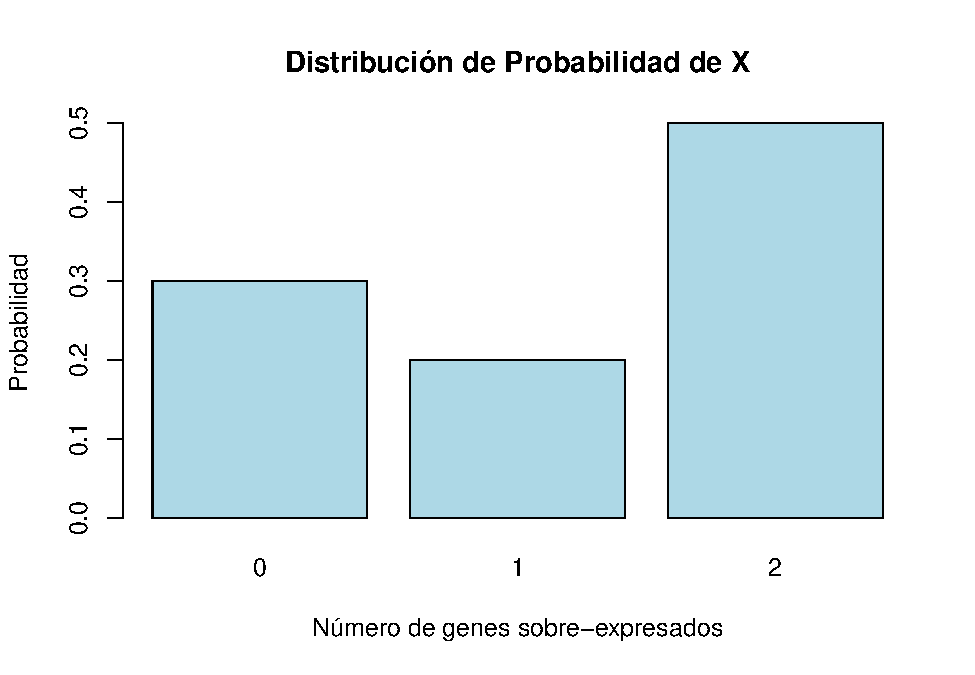
\includegraphics{Ejercicios-de-Inferencia-Estadistica_files/figure-latex/unnamed-chunk-7-1.pdf}

\subsubsection{Esperanza y varianza}\label{esperanza-y-varianza}

La \textbf{esperanza} (o valor esperado) de una variable aleatoria discreta \(X\) se calcula como:

\[
E(X) = \sum_{x} x \cdot P(X = x)
\]

Sustituyendo los valores:

\[
E(X) = 0 \cdot 0.30 + 1 \cdot 0.20 + 2 \cdot 0.50 = 0 + 0.20 + 1.00 = 1.20
\]

La \textbf{varianza} de \(X\) se calcula como:

\[
\text{Var}(X) = E(X^2) - [E(X)]^2
\]

Primero calculamos \(E(X^2)\):

\[
E(X^2) = \sum_{x} x^2 \cdot P(X = x)
\]

\[
E(X^2) = 0^2 \cdot 0.30 + 1^2 \cdot 0.20 + 2^2 \cdot 0.50 = 0 + 0.20 + 2.00 = 2.20
\]

Entonces, la varianza es:

\[
\text{Var}(X) = 2.20 - (1.20)^2 = 2.20 - 1.44 = 0.76
\]

Verificamos los cálculos con R:

\begin{Shaded}
\begin{Highlighting}[]
\CommentTok{\# Calcular esperanza y varianza}
\NormalTok{esperanza }\OtherTok{\textless{}{-}} \FunctionTok{sum}\NormalTok{(X\_values }\SpecialCharTok{*}\NormalTok{ probabilities)}
\NormalTok{esperanza\_cuadrado }\OtherTok{\textless{}{-}} \FunctionTok{sum}\NormalTok{(X\_values}\SpecialCharTok{\^{}}\DecValTok{2} \SpecialCharTok{*}\NormalTok{ probabilities)}

\NormalTok{varianza }\OtherTok{\textless{}{-}}\NormalTok{ esperanza\_cuadrado }\SpecialCharTok{{-}}\NormalTok{ esperanza}\SpecialCharTok{\^{}}\DecValTok{2}

\NormalTok{esperanza}
\end{Highlighting}
\end{Shaded}

\begin{verbatim}
## [1] 1.2
\end{verbatim}

\begin{Shaded}
\begin{Highlighting}[]
\NormalTok{varianza}
\end{Highlighting}
\end{Shaded}

\begin{verbatim}
## [1] 0.76
\end{verbatim}

\subsection{Ejercicio 2.2}\label{ejercicio-2.2}

Para describir el número de mutaciones presentes en un volumen estándar de un tumor unos investigadores han propuesto el modelo siguiente

\[
p(x)=\frac{K}{2+x}, x=0,1,2,3,4,5
\]

\begin{enumerate}
\def\labelenumi{\arabic{enumi}.}
\tightlist
\item
  Determinar qué valor debe de tener \(K\) para que \(p(x)\) sea una función de masa de probabilidad
\item
  Calcular su esperanza y su varianza
\item
  Calcular las probabilidades de los sucesos:

  \begin{itemize}
  \tightlist
  \item
    1 Un tumor presenta exactamente tres mutaciones
  \item
    2 Un tumor presenta al menos una mutación
  \item
    3 Un tumor presenta como máximo dos mutaciones.
  \end{itemize}
\end{enumerate}

\textbf{SOLUCIÓN}

Se considera el modelo para la distribución de probabilidades de mutaciones en un tumor dado por:

\[
p(x)=\frac{K}{2+x}, x=0,1,2,3,4,5
\]

\subsubsection{\texorpdfstring{Valor de \(K\)}{Valor de K}}\label{valor-de-k}

Para que \(p(x)\) sea una función de masa de probabilidad, la suma de todas las probabilidades debe ser igual a 1. Es decir:

\[
\sum_{x=0}^{5} p(x) = 1
\]

Sustituyendo la fórmula de \(p(x)\):

\[
\sum_{x=0}^{5} \frac{K}{2+x} = 1
\]

Simplificamos la suma:

\[
K \sum_{x=0}^{5} \frac{1}{2+x} = 1
\]

La suma es:

\[
\sum_{x=0}^{5} \frac{1}{2+x} = \frac{1}{2} + \frac{1}{3} + \frac{1}{4} + \frac{1}{5} + \frac{1}{6} + \frac{1}{7}
\]

Podemos calcular esta suma numéricamente en R:

\begin{Shaded}
\begin{Highlighting}[]
\CommentTok{\# Valores de la suma}
\NormalTok{suma }\OtherTok{\textless{}{-}} \FunctionTok{sum}\NormalTok{(}\DecValTok{1} \SpecialCharTok{/}\NormalTok{ (}\DecValTok{2} \SpecialCharTok{+} \DecValTok{0}\SpecialCharTok{:}\DecValTok{5}\NormalTok{))}

\CommentTok{\# Calcular el valor de K}
\NormalTok{K }\OtherTok{\textless{}{-}} \DecValTok{1} \SpecialCharTok{/}\NormalTok{ suma}
\NormalTok{K}
\end{Highlighting}
\end{Shaded}

\begin{verbatim}
## [1] 0.6278027
\end{verbatim}

\subsubsection{Esperanza y la varianza}\label{esperanza-y-la-varianza}

La \textbf{esperanza} de \(X\) se calcula como:

\[
E(X) = \sum_{x=0}^{5} x \cdot p(x) = \sum_{x=0}^{5} x \cdot \frac{K}{2+x}
\]

La \textbf{varianza} se calcula usando:

\[
\text{Var}(X) = E(X^2) - [E(X)]^2
\]

Para esto, primero calculamos \(E(X^2)\):

\[
E(X^2) = \sum_{x=0}^{5} x^2 \cdot p(x) = \sum_{x=0}^{5} x^2 \cdot \frac{K}{2+x}
\]

Podemos calcular la esperanza y la varianza en R de la siguiente forma:

\begin{Shaded}
\begin{Highlighting}[]
\CommentTok{\# Calcular la esperanza}
\NormalTok{esperanza }\OtherTok{\textless{}{-}} \FunctionTok{sum}\NormalTok{((}\DecValTok{0}\SpecialCharTok{:}\DecValTok{5}\NormalTok{) }\SpecialCharTok{*}\NormalTok{ K }\SpecialCharTok{/}\NormalTok{ (}\DecValTok{2} \SpecialCharTok{+} \DecValTok{0}\SpecialCharTok{:}\DecValTok{5}\NormalTok{))}

\CommentTok{\# Calcular la esperanza al cuadrado}
\NormalTok{esperanza\_cuadrado }\OtherTok{\textless{}{-}} \FunctionTok{sum}\NormalTok{((}\DecValTok{0}\SpecialCharTok{:}\DecValTok{5}\NormalTok{)}\SpecialCharTok{\^{}}\DecValTok{2} \SpecialCharTok{*}\NormalTok{ K }\SpecialCharTok{/}\NormalTok{ (}\DecValTok{2} \SpecialCharTok{+} \DecValTok{0}\SpecialCharTok{:}\DecValTok{5}\NormalTok{))}

\CommentTok{\# Calcular la varianza}
\NormalTok{varianza }\OtherTok{\textless{}{-}}\NormalTok{ esperanza\_cuadrado }\SpecialCharTok{{-}}\NormalTok{ esperanza}\SpecialCharTok{\^{}}\DecValTok{2}

\NormalTok{esperanza}
\end{Highlighting}
\end{Shaded}

\begin{verbatim}
## [1] 1.766816
\end{verbatim}

\begin{Shaded}
\begin{Highlighting}[]
\NormalTok{varianza}
\end{Highlighting}
\end{Shaded}

\begin{verbatim}
## [1] 2.761769
\end{verbatim}

\subsubsection{Probabilidades}\label{probabilidades}

\textbf{Probabilidad de que un tumor presente exactamente tres mutaciones}

La probabilidad de que \(X = 3\) es:

\[
P(X = 3) = p(3) = \frac{K}{2+3}
\]

Podemos calcularlo en R:

\begin{Shaded}
\begin{Highlighting}[]
\CommentTok{\# Probabilidad de X = 3}
\NormalTok{P\_X\_3 }\OtherTok{\textless{}{-}}\NormalTok{ K }\SpecialCharTok{/}\NormalTok{ (}\DecValTok{2} \SpecialCharTok{+} \DecValTok{3}\NormalTok{)}
\NormalTok{P\_X\_3}
\end{Highlighting}
\end{Shaded}

\begin{verbatim}
## [1] 0.1255605
\end{verbatim}

\textbf{Probabilidad de que un tumor presente al menos una mutación}

La probabilidad de que \(X \geq 1\) es:

\[
P(X \geq 1) = 1 - P(X = 0)
\]

Podemos calcularlo en R:

\begin{Shaded}
\begin{Highlighting}[]
\CommentTok{\# Probabilidad de X \textgreater{}= 1}
\NormalTok{P\_X\_1 }\OtherTok{\textless{}{-}} \DecValTok{1} \SpecialCharTok{{-}}\NormalTok{ K }\SpecialCharTok{/}\NormalTok{ (}\DecValTok{2} \SpecialCharTok{+} \DecValTok{0}\NormalTok{)}
\NormalTok{P\_X\_1}
\end{Highlighting}
\end{Shaded}

\begin{verbatim}
## [1] 0.6860987
\end{verbatim}

\textbf{Probabilidad de que un tumor presente como máximo dos mutaciones}

La probabilidad de que \(X \leq 2\) es:

\[
P(X \leq 2) = P(X = 0) + P(X = 1) + P(X = 2)
\]

Podemos calcularlo en R:

\begin{Shaded}
\begin{Highlighting}[]
\CommentTok{\# Probabilidad de X \textless{}= 2}
\NormalTok{P\_X\_2 }\OtherTok{\textless{}{-}} \FunctionTok{sum}\NormalTok{(K }\SpecialCharTok{/}\NormalTok{ (}\DecValTok{2} \SpecialCharTok{+} \DecValTok{0}\SpecialCharTok{:}\DecValTok{2}\NormalTok{))}
\NormalTok{P\_X\_2}
\end{Highlighting}
\end{Shaded}

\begin{verbatim}
## [1] 0.6801196
\end{verbatim}

\subsection{Ejercicio 2.3}\label{ejercicio-2.3}

Un modelo simplificado del tiempo de supervivencia, en años, tras un diagnóstico de una variante de leucemia es el siguiente:

\[
f_{x}(x)=-0.5 \cdot x+1, \quad \text { donde } \quad 0 \leq x \leq 2
\]

\begin{enumerate}
\def\labelenumi{\arabic{enumi}.}
\item
  Comprobar que \(f_{X}\) es una densidad. Representarla gráficamente.
\item
  Calcular \(\mathrm{F}_{\mathrm{X}} \mathrm{y}\) representarla gráficamente.
\item
  Calcular \(P(X \geq 1), P(X>1), P(X=1), f_{x}(1)\).
\item
  Calcular la probabilidad de que un individuo diagnosticado con leucemia sobreviva :
\end{enumerate}

\begin{enumerate}
\def\labelenumi{(\roman{enumi})}
\tightlist
\item
  menos de seis meses, (ii) entre seis meses y un año, (iii) más de dos años.
\end{enumerate}

\begin{enumerate}
\def\labelenumi{\arabic{enumi}.}
\setcounter{enumi}{4}
\item
  Calcular \(E(X)\) i \(\operatorname{Var}(X)\).
\item
  En vista que el modelo anterior no ha resultado satisfactorio una bioestadística ha propuesto un modelo alternativo consistente en modelizar la variable como:
\end{enumerate}

\[
g_{X}(x)=\exp (-k x), \text { dondex } \geq 0
\]

Calcular la constante \(k\) para que \(\mathrm{g}_{\mathrm{x}}\) sea una función de densidad de probabilidad. Repetir los cálculos de los apartados b), c), d) y e) con el nuevo modelo. Discutir adecuación de ambos modelos a una situación real.

\textbf{SOLUCIÓN}

\subsubsection{\texorpdfstring{\(f_X(x)\) es una densidad}{f\_X(x) es una densidad}}\label{f_xx-es-una-densidad}

Para comprobar que \(f_X(x)\) es una función de densidad, necesitamos verificar que cumple las dos condiciones básicas:

\begin{enumerate}
\def\labelenumi{\arabic{enumi}.}
\tightlist
\item
  \(f_X(x) \geq 0\) para todo \(x\) en su dominio.
\item
  La integral de \(f_X(x)\) sobre todo su dominio debe ser 1, es decir:
\end{enumerate}

\[
\int_0^2 f_X(x) \, dx = 1
\]

La función de densidad dada es \(f_X(x) = -0.5 \cdot x + 1\) con \(0 \leq x \leq 2\).

Primero, comprobamos que \(f_X(x) \geq 0\) para \(x \in [0, 2]\). Evaluamos los valores extremos:

\begin{itemize}
\tightlist
\item
  \(f_X(0) = -0.5 \cdot 0 + 1 = 1\)
\item
  \(f_X(2) = -0.5 \cdot 2 + 1 = 0\)
\end{itemize}

La función es no negativa en el intervalo dado.

Ahora, calculamos la integral:

\[
\int_0^2 (-0.5 \cdot x + 1) \, dx = \left[ -0.25 \cdot x^2 + x \right]_0^2 = (-0.25 \cdot 4 + 2) - (0) = 1
\]

Por lo tanto, \(f_X(x)\) cumple con ambas condiciones y es una función de densidad.

\subsubsection{\texorpdfstring{Gráfica de \(f_X(x)\)}{Gráfica de f\_X(x)}}\label{gruxe1fica-de-f_xx}

\begin{Shaded}
\begin{Highlighting}[]
\CommentTok{\# R code to plot the density function}
\NormalTok{f\_x }\OtherTok{\textless{}{-}} \ControlFlowTok{function}\NormalTok{(x) }\SpecialCharTok{{-}}\FloatTok{0.5} \SpecialCharTok{*}\NormalTok{ x }\SpecialCharTok{+} \DecValTok{1}
\FunctionTok{curve}\NormalTok{(f\_x, }\AttributeTok{from =} \DecValTok{0}\NormalTok{, }\AttributeTok{to =} \DecValTok{2}\NormalTok{, }\AttributeTok{col =} \StringTok{"blue"}\NormalTok{, }\AttributeTok{lwd =} \DecValTok{2}\NormalTok{, }\AttributeTok{ylab =} \StringTok{"f\_X(x)"}\NormalTok{, }\AttributeTok{xlab =} \StringTok{"x"}\NormalTok{,}
      \AttributeTok{main =} \StringTok{"Densidad f\_X(x)"}\NormalTok{)}
\end{Highlighting}
\end{Shaded}

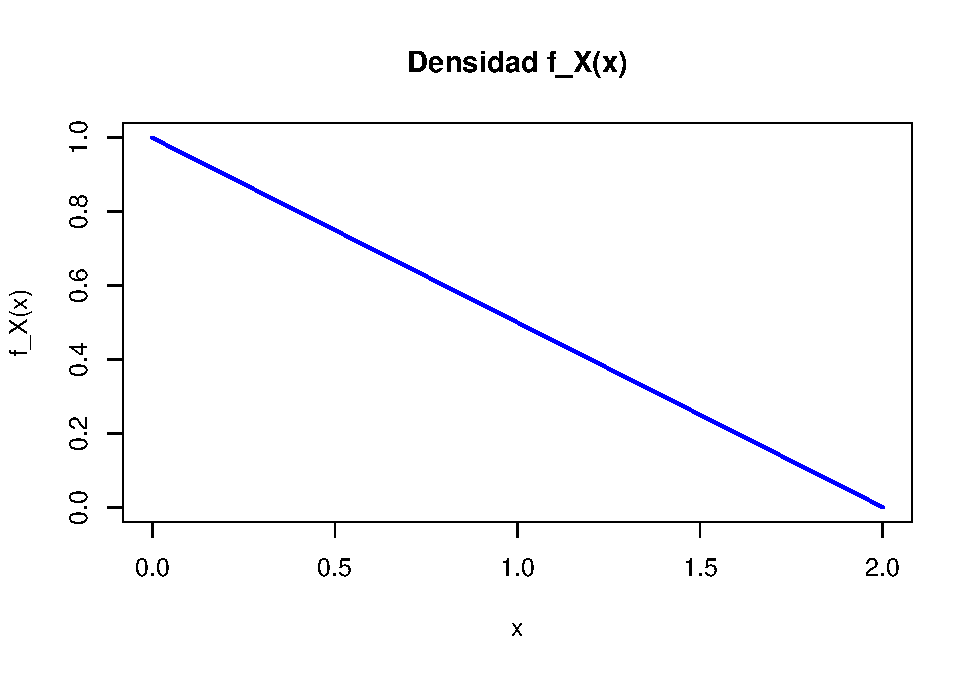
\includegraphics{Ejercicios-de-Inferencia-Estadistica_files/figure-latex/unnamed-chunk-14-1.pdf}

\subsubsection{Función de distribución}\label{funciuxf3n-de-distribuciuxf3n}

\textbf{Calcular \(F_X(x)\) y representarla gráficamente}

La función de distribución acumulada (CDF) \(F_X(x)\) se obtiene integrando la función de densidad:

\[
F_X(x) = \int_0^x (-0.5 \cdot t + 1) \, dt
\]

Para \(x \in [0, 2]\), tenemos:

\[
F_X(x) = \left[-0.25 \cdot t^2 + t\right]_0^x = -0.25 \cdot x^2 + x
\]

Para \(x < 0\), \(F_X(x) = 0\), y para \(x > 2\), \(F_X(x) = 1\).

\textbf{Gráfica de \(F_X(x)\)ç}

\begin{Shaded}
\begin{Highlighting}[]
\CommentTok{\# R code to plot the CDF function}
\NormalTok{F\_x }\OtherTok{\textless{}{-}} \ControlFlowTok{function}\NormalTok{(x) }\FunctionTok{ifelse}\NormalTok{(x }\SpecialCharTok{\textless{}} \DecValTok{0}\NormalTok{, }\DecValTok{0}\NormalTok{, }\FunctionTok{ifelse}\NormalTok{(x }\SpecialCharTok{\textgreater{}} \DecValTok{2}\NormalTok{, }\DecValTok{1}\NormalTok{, }\SpecialCharTok{{-}}\FloatTok{0.25} \SpecialCharTok{*}\NormalTok{ x}\SpecialCharTok{\^{}}\DecValTok{2} \SpecialCharTok{+}\NormalTok{ x))}
\FunctionTok{curve}\NormalTok{(F\_x, }\AttributeTok{from =} \SpecialCharTok{{-}}\DecValTok{1}\NormalTok{, }\AttributeTok{to =} \DecValTok{3}\NormalTok{, }\AttributeTok{col =} \StringTok{"red"}\NormalTok{, }\AttributeTok{lwd =} \DecValTok{2}\NormalTok{, }\AttributeTok{ylab =} \StringTok{"F\_X(x)"}\NormalTok{, }\AttributeTok{xlab =} \StringTok{"x"}\NormalTok{,}
      \AttributeTok{main =} \StringTok{"Distribución acumulada F\_X(x)"}\NormalTok{)}
\end{Highlighting}
\end{Shaded}

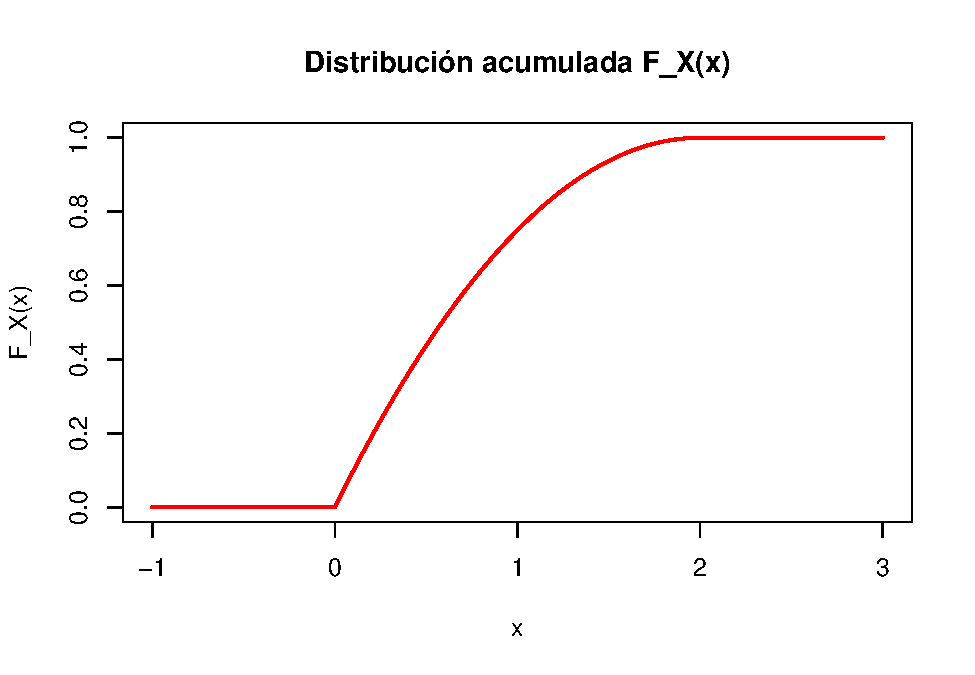
\includegraphics{Ejercicios-de-Inferencia-Estadistica_files/figure-latex/unnamed-chunk-15-1.pdf}

\subsubsection{\texorpdfstring{Probabilidades y \(f_X(1)\)}{Probabilidades y f\_X(1)}}\label{probabilidades-y-f_x1}

\begin{enumerate}
\def\labelenumi{\arabic{enumi}.}
\tightlist
\item
  \(P(X \geq 1) = 1 - F_X(1)\):
\end{enumerate}

\[
F_X(1) = -0.25 \cdot 1^2 + 1 = 0.75
\]
Por lo tanto, \(P(X \geq 1) = 1 - 0.75 = 0.25\).

\begin{enumerate}
\def\labelenumi{\arabic{enumi}.}
\setcounter{enumi}{1}
\item
  \(P(X > 1)\): Como \(X\) es una variable continua, \(P(X > 1) = P(X \geq 1) = 0.25\).
\item
  \(P(X = 1)\): Para una variable continua, la probabilidad puntual es 0, es decir, \(P(X = 1) = 0\).
\item
  \(f_X(1)\):
\end{enumerate}

\[
f_X(1) = -0.5 \cdot 1 + 1 = 0.5
\]

\subsubsection{Probabilidad de supervivencia}\label{probabilidad-de-supervivencia}

\begin{enumerate}
\def\labelenumi{\arabic{enumi}.}
\tightlist
\item
  Menos de seis meses (\(x = 0.5\)):
\end{enumerate}

\[
P(X < 0.5) = F_X(0.5) = -0.25 \cdot 0.5^2 + 0.5 = 0.375
\]

\begin{enumerate}
\def\labelenumi{\arabic{enumi}.}
\setcounter{enumi}{1}
\tightlist
\item
  Entre seis meses y un año (\(x \in [0.5, 1]\)):
\end{enumerate}

\[
P(0.5 \leq X \leq 1) = F_X(1) - F_X(0.5) = 0.75 - 0.375 = 0.375
\]

\begin{enumerate}
\def\labelenumi{\arabic{enumi}.}
\setcounter{enumi}{2}
\tightlist
\item
  Más de dos años (\(x > 2\)): Como el dominio de \(X\) es \([0, 2]\), \(P(X > 2) = 0\).
\end{enumerate}

\subsubsection{\texorpdfstring{\(E(X)\) y \(\operatorname{Var}(X)\)}{E(X) y \textbackslash operatorname\{Var\}(X)}}\label{ex-y-operatornamevarx}

\begin{enumerate}
\def\labelenumi{\arabic{enumi}.}
\tightlist
\item
  La esperanza de \(X\) es:
\end{enumerate}

\[
E(X) = \int_0^2 x \cdot f_X(x) \, dx = \int_0^2 x \cdot (-0.5 \cdot x + 1) \, dx
\]

Desarrollamos:

\[
E(X) = \int_0^2 (-0.5 \cdot x^2 + x) \, dx = \left[-\frac{0.5}{3} \cdot x^3 + 0.5 \cdot x^2\right]_0^2
\]

Calculamos:

\[
E(X) = -\frac{0.5}{3} \cdot 8 + 0.5 \cdot 4 = -\frac{4}{3} + 2 = \frac{2}{3}
\]

\begin{enumerate}
\def\labelenumi{\arabic{enumi}.}
\setcounter{enumi}{1}
\tightlist
\item
  La varianza de \(X\) es:
\end{enumerate}

\[
\operatorname{Var}(X) = E(X^2) - E(X)^2
\]

Primero calculamos \(E(X^2)\):

\[
E(X^2) = \int_0^2 x^2 \cdot f_X(x) \, dx = \int_0^2 x^2 \cdot (-0.5 \cdot x + 1) \, dx
\]

Desarrollamos y calculamos:

\[
E(X^2) = \int_0^2 (-0.5 \cdot x^3 + x^2) \, dx = \left[-\frac{0.5}{4} \cdot x^4 + \frac{1}{3} \cdot x^3\right]_0^2
\]

\[
E(X^2) = -\frac{0.5}{4} \cdot 16 + \frac{1}{3} \cdot 8 = -2 + \frac{8}{3} = \frac{2}{3}
\]

Finalmente:

\[
\operatorname{Var}(X) = E(X^2) - E(X)^2 = \frac{2}{3} - \left(\frac{2}{3}\right)^2 = \frac{2}{3} - \frac{4}{9} = \frac{2}{9}
\]

\subsubsection{\texorpdfstring{Modelo alternativo \(g_X(x)\)}{Modelo alternativo g\_X(x)}}\label{modelo-alternativo-g_xx}

Dado el modelo alternativo \(g_X(x) = \exp(-k \cdot x)\) para \(x \geq 0\), la constante \(k\) se determina imponiendo que la integral de la función de densidad debe ser 1:

\[
\int_0^\infty \exp(-k \cdot x) \, dx = 1
\]

Resolviendo:

\[
\frac{1}{k} = 1 \implies k = 1
\]

Por lo tanto, el nuevo modelo de densidad es \(g_X(x) = \exp(-x)\).

\subsection{Ejercicio 2.4}\label{ejercicio-2.4}

Para estudiar la regulación hormonal de una línea metabólica se inyectan ratas albinas con un fármaco que inhibe la síntesis de proteínas del organismo. En general, 4 de cada 20 ratas mueren a causa del fármaco antes de que el experimento haya concluido. Si se trata a 10 animales con el fármaco, ¿cuál es la probabilidad de que al menos 8 lleguen vivas al final del experimento?

\textbf{SOLUCION}

En este problema en el que tenemos grupos de 10 animales independientes, cada uno de los cuales puede sobrevivir o no resulta apropiada \textbf{la distribución binomial}.

\begin{itemize}
\item
  La probabilidad de que una rata sobreviva al fármaco es \(p = \frac{16}{20} = 0.8\), dado que 4 de cada 20 ratas mueren.
\item
  El experimento se realiza con 10 ratas, por lo que tenemos \(n = 10\).
\item
  Queremos calcular la probabilidad de que al menos 8 ratas sobrevivan. Matemáticamente, esto corresponde a:
\end{itemize}

\[
P(X \geq 8)
\]

donde \(X\) es el número de ratas que sobreviven y sigue una \textbf{distribución binomial}:

\[
X \sim \text{Binomial}(n=10, p=0.8)
\]

\subsubsection{Cálculo de la probabilidad}\label{cuxe1lculo-de-la-probabilidad}

La probabilidad de que exactamente \(k\) ratas sobrevivan está dada por la fórmula de la binomial:

\[
P(X = k) = \binom{n}{k} p^k (1 - p)^{n-k}
\]

Para responder la pregunta debemos calcular:

\[
P(X \geq 8) = P(X = 8) + P(X = 9) + P(X = 10)
\]
Esto puede calcularse:

\begin{itemize}
\tightlist
\item
  directamente usando la función de probabilidad acumulada implementada en R
\item
  indirectamente calculando las probabilidades individuales y sumándolas.
\end{itemize}

En todo caso debemos recordar que al tratarse de una variable discreta si queremos usar \(F_X(x)\) para calcular \(P(X\geq k)\) deberemos tener en cuenta que:
\[
P(X\geq k) = 1-P(X\leq k-1)
\]
En primer lugar calculamos esta suma utilizando la función de masa de probabilidad:

\begin{Shaded}
\begin{Highlighting}[]
\CommentTok{\# Parámetros del problema}
\NormalTok{n }\OtherTok{\textless{}{-}} \DecValTok{10}
\NormalTok{p }\OtherTok{\textless{}{-}} \FloatTok{0.8}

\CommentTok{\# Probabilidades P(X = 8), P(X = 9) y P(X = 10)}
\NormalTok{prob\_8 }\OtherTok{\textless{}{-}} \FunctionTok{dbinom}\NormalTok{(}\DecValTok{8}\NormalTok{, }\AttributeTok{size =}\NormalTok{ n, }\AttributeTok{prob =}\NormalTok{ p)}
\NormalTok{prob\_9 }\OtherTok{\textless{}{-}} \FunctionTok{dbinom}\NormalTok{(}\DecValTok{9}\NormalTok{, }\AttributeTok{size =}\NormalTok{ n, }\AttributeTok{prob =}\NormalTok{ p)}
\NormalTok{prob\_10 }\OtherTok{\textless{}{-}} \FunctionTok{dbinom}\NormalTok{(}\DecValTok{10}\NormalTok{, }\AttributeTok{size =}\NormalTok{ n, }\AttributeTok{prob =}\NormalTok{ p)}

\CommentTok{\# Probabilidad total P(X \textgreater{}= 8)}
\NormalTok{prob\_total }\OtherTok{\textless{}{-}}\NormalTok{ prob\_8 }\SpecialCharTok{+}\NormalTok{ prob\_9 }\SpecialCharTok{+}\NormalTok{ prob\_10}
\NormalTok{prob\_total}
\end{Highlighting}
\end{Shaded}

\begin{verbatim}
## [1] 0.6777995
\end{verbatim}

Si usamos la funcion de distribución, \texttt{pbinom}

\begin{Shaded}
\begin{Highlighting}[]
\DecValTok{1}\SpecialCharTok{{-}}\FunctionTok{pbinom}\NormalTok{ (}\DecValTok{7}\NormalTok{, }\AttributeTok{size =}\NormalTok{ n, }\AttributeTok{prob =}\NormalTok{ p)}
\end{Highlighting}
\end{Shaded}

\begin{verbatim}
## [1] 0.6777995
\end{verbatim}

Naturalmente ambos resultados coinciden. Obsérvese que al ser \(p=0.8\) valores altos resultan bastante probables, con lo que la

\subsection{Ejercicio 2.5}\label{ejercicio-2.5}

En una cierta población se ha observado un número medio anual de 12 muertes por cáncer de pulmón. Si el número de muertes causadas por la enfermedad sigue una distribución de Poisson, ¿cuál es la probabilidad de que durante el año en curso:
1. haya exactamente 10 muertes por cáncer de pulmón?
2. 15 o más personas mueran a causa de la enfermedad?
3. 10 o menos personas mueran a causa de la enfermedad?

El número de muertes por cáncer de pulmón sigue una distribución de Poisson, que se usa para modelar la ocurrencia de eventos discretos dentro de un intervalo de tiempo, donde el valor esperado es proporcional al tamaño del intervalo. En este caso, el valor esperado es el número medio de muertes por año, que es 12. La función de masa de probabilidad (PMF) de una variable aleatoria \(X\) con distribución de Poisson y parámetro \(\lambda\) es:

\[ P(X = k) = \frac{\lambda^k e^{-\lambda}}{k!} \]

donde \(k\) es el número de eventos, \(\lambda\) es el valor esperado (12 en nuestro caso) y \(k!\) es el factorial de \(k\). Usaremos este modelo para resolver los apartados.

\subsubsection{Probabilidad de que haya exactamente 10 muertes}\label{probabilidad-de-que-haya-exactamente-10-muertes}

La probabilidad de observar exactamente \(k = 10\) muertes se puede calcular usando la PMF de la distribución de Poisson con \(\lambda = 12\):

\[ P(X = 10) = \frac{12^{10} e^{-12}}{10!} \]

Podemos calcular este valor con R.

\begin{Shaded}
\begin{Highlighting}[]
\NormalTok{lambda }\OtherTok{\textless{}{-}} \DecValTok{12}
\NormalTok{k }\OtherTok{\textless{}{-}} \DecValTok{10}
\NormalTok{prob\_10\_muertes }\OtherTok{\textless{}{-}} \FunctionTok{dpois}\NormalTok{(k, lambda)}
\NormalTok{prob\_10\_muertes}
\end{Highlighting}
\end{Shaded}

\begin{verbatim}
## [1] 0.1048373
\end{verbatim}

\subsubsection{Probabilidad de que 15 o más personas mueran}\label{probabilidad-de-que-15-o-muxe1s-personas-mueran}

Para obtener la probabilidad de que 15 o más personas mueran, necesitamos calcular la probabilidad acumulada de \(X \geq 15\). Esto se puede obtener restando de 1 la probabilidad acumulada de \(X < 15\), es decir:

\[ P(X \geq 15) = 1 - P(X < 15) = 1 - P(X \leq 14) \]

Usamos la función de probabilidad acumulada (CDF) de la Poisson en R.

\begin{Shaded}
\begin{Highlighting}[]
\NormalTok{k\_15 }\OtherTok{\textless{}{-}} \DecValTok{14}
\NormalTok{prob\_15\_o\_mas }\OtherTok{\textless{}{-}} \DecValTok{1} \SpecialCharTok{{-}} \FunctionTok{ppois}\NormalTok{(k\_15, lambda)}
\NormalTok{prob\_15\_o\_mas}
\end{Highlighting}
\end{Shaded}

\begin{verbatim}
## [1] 0.2279755
\end{verbatim}

\subsubsection{Probabilidad de que 10 o menos personas mueran}\label{probabilidad-de-que-10-o-menos-personas-mueran}

La probabilidad de que 10 o menos personas mueran es simplemente la probabilidad acumulada de \(X \leq 10\), que se puede calcular directamente con la CDF de la distribución de Poisson.

\[ P(X \leq 10) \]

Calculamos esto en R:

\begin{Shaded}
\begin{Highlighting}[]
\NormalTok{prob\_10\_o\_menos }\OtherTok{\textless{}{-}} \FunctionTok{ppois}\NormalTok{(k, lambda)}
\NormalTok{prob\_10\_o\_menos}
\end{Highlighting}
\end{Shaded}

\begin{verbatim}
## [1] 0.3472294
\end{verbatim}

\subsubsection{Conclusión}\label{conclusiuxf3n}

\begin{enumerate}
\def\labelenumi{\arabic{enumi}.}
\tightlist
\item
  La probabilidad de que haya exactamente 10 muertes es:
\end{enumerate}

\begin{Shaded}
\begin{Highlighting}[]
\NormalTok{prob\_10\_muertes}
\end{Highlighting}
\end{Shaded}

\begin{verbatim}
## [1] 0.1048373
\end{verbatim}

\begin{enumerate}
\def\labelenumi{\arabic{enumi}.}
\setcounter{enumi}{1}
\tightlist
\item
  La probabilidad de que 15 o más personas mueran es:
\end{enumerate}

\begin{Shaded}
\begin{Highlighting}[]
\NormalTok{prob\_15\_o\_mas}
\end{Highlighting}
\end{Shaded}

\begin{verbatim}
## [1] 0.2279755
\end{verbatim}

\begin{enumerate}
\def\labelenumi{\arabic{enumi}.}
\setcounter{enumi}{2}
\tightlist
\item
  La probabilidad de que 10 o menos personas mueran es:
\end{enumerate}

\begin{Shaded}
\begin{Highlighting}[]
\NormalTok{prob\_10\_o\_menos}
\end{Highlighting}
\end{Shaded}

\begin{verbatim}
## [1] 0.3472294
\end{verbatim}

\subsection{Ejercicio 2.6}\label{ejercicio-2.6}

Los daños a los cromosomas del óvulo o del espermatozoide, pueden causar mutaciones que conducen a abortos, defectos de nacimiento, u otras deficiencias genéticas. Un estudio sobre los efectos teratogénicos de la radiación ha determinado que la probabilidad de que tal mutación se produzca por radiación es del 10\%. El resto son atribuibles a otras causas.
Una vez detectadas 150 mutaciones,

\begin{enumerate}
\def\labelenumi{\arabic{enumi}.}
\tightlist
\item
  ¿cuántas se esperaría que se debiesen a radiaciones?
\item
  ¿Cuál es la probabilidad de que solamente 10 se debiesen a radiaciones?
\end{enumerate}

\textbf{Solución}

Para analizar el número de mutaciones que se deben a radiaciones, podemos considera dos modelos diferentes: uno basado en la distribución binomial y otro en la distribución de Poisson.

\subsubsection{Justificación del uso de distribución binomial}\label{justificaciuxf3n-del-uso-de-distribuciuxf3n-binomial}

La distribución binomial es adecuada cuando tenemos un número fijo de ensayos independientes y cada ensayo tiene dos posibles resultados: éxito (la mutación es debida a radiación) o fracaso (la mutación no es debida a radiación). En cada ensayo, la probabilidad de éxito es constante.

Esto se ajusta perfectamente a las condiciones del problema:
- Hay 150 ensayos independientes (cada mutación observada puede estar o no causada por radiación).
- Cada ensayo tiene dos posibles resultados: mutación por radiación o mutación por otra causa.
- La probabilidad de éxito es constante y pequeña (\(p = 0.1\)).
Por tanto, el número de mutaciones debidas a radiación se puede modelizar bien mediante una distribución binomial \(X \sim \text{Binomial}(n = 150, p = 0.1)\).

\subsubsection{Justificación del uso de distribución de Poisson}\label{justificaciuxf3n-del-uso-de-distribuciuxf3n-de-poisson}

La distribución de Poisson es adecuada para modelar el número de eventos raros que ocurren en un intervalo de tiempo, espacio, o cualquier otra unidad, cuando estos eventos ocurren de forma independiente y su probabilidad de ocurrencia es baja.

En este caso las ``mutaciones debidas a radiación'' pueden considerarse eventos raros dentro de un gran conjunto de mutaciones (150 mutaciones observadas, pero solo un 10\% de ellas son debidas a radiación).

Puede considerarse además, que las mutaciones individuales pueden ocurrir de forma independiente entre sí, ya que la probabilidad de que una mutación se deba a radiación no afecta a la probabilidad de que otra mutación sea causada por radiación.

Estas condiciones son características de los \emph{procesos de Poisson} y por tanto la distribución de Poisson es una elección natural para describir procesos en los que los eventos ocurren de manera aleatoria en un intervalo dado (por ejemplo, en un periodo de tiempo o un espacio), siempre que:

\begin{itemize}
\tightlist
\item
  Los eventos ocurran con una tasa promedio constante (en este caso, la tasa de mutaciones debidas a radiaciones es proporcional a la tasa global de mutaciones, multiplicada por la probabilidad \(p = 0.1\)).
\item
  No haya límite teórico en el número de eventos que puedan ocurrir en un intervalo (aunque observamos un total de 150 mutaciones, teóricamente podríamos seguir detectando más mutaciones).
\end{itemize}

En el modelo de Poisson, el parámetro \(\lambda\) representa la tasa promedio de ocurrencia de los eventos (en este caso, mutaciones debidas a radiación). Si conocemos la tasa promedio de aparición de mutaciones por radiación (\(\lambda = n \cdot p\) en el contexto binomial, pero también se puede calcular directamente si conocemos la tasa de aparición de eventos raros), entonces podemos usar directamente la distribución de Poisson para modelar el número de eventos.

En este caso, \(\lambda = 150 \cdot 0.1 = 15\), que representa el número esperado de mutaciones debidas a radiación en el total observado de mutaciones.

\subsubsection{Aproximación del modelo binomial por el de Poisson}\label{aproximaciuxf3n-del-modelo-binomial-por-el-de-poisson}

La distribución de Poisson puede considerarse una aproximación de la binomial cuando el número de ensayos (\(n\)) es grande y la probabilidad de éxito (\(p\)) es pequeña. En este caso, el número esperado de éxitos, \(n \cdot p\), se mantiene moderado (en este caso, \(n \cdot p = 15\)).

Este resultado que se conoce como \emph{límite de Poisson} establece que si:

\begin{itemize}
\tightlist
\item
  \(n\) es grande (muchos ensayos),
\item
  \(p\) es pequeño (baja probabilidad de éxito),
\item
  el producto \(n \cdot p = \lambda\) es moderado,
\end{itemize}

entonces la binomial \(X \sim \text{Binomial}(n, p)\) se puede aproximar por una distribución de Poisson con parámetro \(\lambda = n \cdot p\).

En este caso:

\begin{itemize}
\tightlist
\item
  \(n = 150\) es suficientemente grande.
\item
  \(p = 0.1\) es pequeño.
\item
  \(n \cdot p = 15\), lo cual es un valor razonable para usar la aproximación de Poisson.
\end{itemize}

Por tanto, el número de mutaciones debidas a radiaciones puede aproximarse por una distribución de Poisson \(X \sim \text{Poisson}(\lambda = 15)\).

\subsubsection{Número esperado de mutaciones}\label{nuxfamero-esperado-de-mutaciones}

En ambos modelos, la esperanza del número de mutaciones debidas a radiaciones es \(E[X] = n \cdot p\). Esto representa el número promedio de mutaciones debidas a radiaciones. Lo calculamos:

\[ E[X] = 150 \cdot 0.1 = 15 \]

Por lo tanto, se espera que alrededor de 15 mutaciones se deban a radiaciones.

\subsubsection{Probabilidad de que exactamente 10 mutaciones se deban a radiaciones}\label{probabilidad-de-que-exactamente-10-mutaciones-se-deban-a-radiaciones}

\paragraph{Usando la distribución Binomial}\label{usando-la-distribuciuxf3n-binomial}

La probabilidad de que exactamente 10 mutaciones se deban a radiaciones se puede calcular usando la PMF de la binomial:

\[ P(X = 10) = \binom{150}{10} (0.1)^{10} (0.9)^{140} \]

Usando R tenemos:

\begin{Shaded}
\begin{Highlighting}[]
\NormalTok{n }\OtherTok{\textless{}{-}} \DecValTok{150}
\NormalTok{p }\OtherTok{\textless{}{-}} \FloatTok{0.1}
\NormalTok{k }\OtherTok{\textless{}{-}} \DecValTok{10}
\NormalTok{prob\_binom\_10 }\OtherTok{\textless{}{-}} \FunctionTok{dbinom}\NormalTok{(k, n, p)}
\NormalTok{prob\_binom\_10}
\end{Highlighting}
\end{Shaded}

\begin{verbatim}
## [1] 0.04591681
\end{verbatim}

\paragraph{Usando la aproximación de Poisson}\label{usando-la-aproximaciuxf3n-de-poisson}

La distribución de Poisson con \(\lambda = n \cdot p = 15\) también se puede usar para aproximar esta probabilidad. La probabilidad de obtener exactamente 10 mutaciones se calcula como:

\[ P(X = 10) = \frac{15^{10} e^{-15}}{10!} \]

Con R:

\begin{Shaded}
\begin{Highlighting}[]
\NormalTok{lambda }\OtherTok{\textless{}{-}} \DecValTok{15}
\NormalTok{prob\_pois\_10 }\OtherTok{\textless{}{-}} \FunctionTok{dpois}\NormalTok{(k, lambda)}
\NormalTok{prob\_pois\_10}
\end{Highlighting}
\end{Shaded}

\begin{verbatim}
## [1] 0.04861075
\end{verbatim}

\subsubsection{Conclusión}\label{conclusiuxf3n-1}

\begin{itemize}
\item
  Se espera que 15 de las 150 mutaciones se deban a radiaciones.
\item
  La probabilidad de que exactamente 10 mutaciones se deban a radiaciones es:

  \begin{itemize}
  \tightlist
  \item
    Usando la distribución binomial:
  \end{itemize}

\begin{Shaded}
\begin{Highlighting}[]
\NormalTok{prob\_binom\_10}
\end{Highlighting}
\end{Shaded}

\begin{verbatim}
## [1] 0.04591681
\end{verbatim}

  \begin{itemize}
  \tightlist
  \item
    Usando la aproximación de Poisson:
  \end{itemize}

\begin{Shaded}
\begin{Highlighting}[]
\NormalTok{prob\_pois\_10}
\end{Highlighting}
\end{Shaded}

\begin{verbatim}
## [1] 0.04861075
\end{verbatim}
\end{itemize}

Ambos métodos dan resultados similares, pero el modelo de Poisson es útil para simplificar los cálculos cuando el número total de mutaciones es grande y la probabilidad de cada evento es pequeña.

\subsection{Ejercicio 2.7}\label{ejercicio-2.7}

Entre los diabéticos, el nivel de glucosa en sangre \(X\), en ayunas, puede suponerse de distribución aproximadamente normal, con media \(106 \mathrm{mg} / 100 \mathrm{ml}\) y desviación típica \(8 \mathrm{mg} / 100 \mathrm{ml}\), es decir : \(X \sim N\left(\mu=106, \sigma^{2}=64\right)\).

Hallar
a) El porcentaje de diabéticos con niveles de glucosa inferiores a 120 ( \(P[X \leq 120]\)
b) ¿Qué porcentaje de diabéticos tienen niveles comprendidos entre 90 y 120?
c) Hallar el nivel de glucosa ``p25'', caracterizado por la propiedad de que el \(25 \%\) de todos los diabéticos tiene un nivel de glucosa en ayunas inferior o igual a \(x\).

\subsection{Ejercicio 28}\label{ejercicio-28}

Se supone que la glucemia basal en individuos sanos, \(X_{s}\) sigue una distribución \(X \sim N(\mu=80, \sigma=10)\), mientras que en los diabéticos \(X_{d}\), sigue una distribución \(X \sim N(\mu=160, \sigma=31.4)\). Si se conviene en clasificar como sanos al \(2 \%\) de los diabéticos:
a) ¿Por debajo de qué valor se considera sano a un individuo? ¿Cuántos sanos serán clasificados como diabéticos?
b) Se sabe que en la población en general el \(10 \%\) de los individuos son diabéticos ¿cuál es la probabilidad de que un individuo elegido al azar y diagnosticado como diabético, realmente lo sea?

\subsection{Ejercicio 2.9}\label{ejercicio-2.9}

Supóngase que se van a utilizar 20 ratas en un estudio de agentes coagulantes de la sangre. Como primera experiencia, se dio un anticoagulante a 10 de ellos, pero por inadvertencia se pusieron todas sin marcas en el mismo recinto. Se necesitaron 12 ratas para la segunda fase del estudio y se le tomó al azar sin reemplazamiento. ¿Cuál es la probabilidad de que de las 12 elegidas 6 tengan la droga y 6 no la tengan?

\section{Distribuciones de probabilidad multidimensionales}\label{distribuciones-de-probabilidad-multidimensionales}

\subsection{Ejercicio 1}\label{ejercicio-1}

Se tienen dos estudios clínicos importantes, cuyos análisis genéticos deben ser asignados aleatoriamente a uno o más de tres laboratorios, A, B y C. Denote con \(Y_{1}\) el número de estudios asignados al laboratorio A y con \(Y_{2}\) el número de estudios asignados al laboratorio B. Cada laboratorio puede recibir 0, 1 o 2 estudios.

\begin{enumerate}
\def\labelenumi{\alph{enumi}.}
\item
  Encuentre la función de probabilidad conjunta para \(Y_{1}\) y \(Y_{2}\).
\item
  Encuentre \(F(1,0)\), es decir, la probabilidad de que el laboratorio A reciba como máximo un estudio y el laboratorio B no reciba ninguno.
\end{enumerate}

\subsection{Ejercicio 2}\label{ejercicio-2}

Tres monedas balanceadas se lanzan en forma independiente al aire. Una de las variables de interés es \(Y_{1}\), el número de caras. Denote con \(Y_{2}\) la cantidad de dinero ganado en una apuesta colateral en la siguiente forma. Si la primera cara aparece en el primer tiro, usted gana 1€. Si la primera cara aparece en el tiro segundo o en el tercero gana 2€ o 3€, respectivamente. Si no aparece una cara, usted pierde 1€ (esto es, gana - 1€ ).
a Encuentre la función de probabilidad conjunta para \(Y_{1}\) y \(Y_{2}\).
b ¿Cuál es la probabilidad de que haya menos de tres caras y usted gane 1€ o menos? {[}Esto es, encuentre \(F(2,1)\).

\subsection{Ejercicio 3}\label{ejercicio-3}

En el Ejercicio 1 determinamos que la distribución conjunta de \(Y_{1}\), el número de análisis asignados al laboratorio A, y \(Y_{2}\), el número de análisis asignados al laboratorio B , está dada por las entradas en la siguiente tabla.

\begin{longtable}[]{@{}cccc@{}}
\toprule\noalign{}
& \(y_{1}\) & & \\
\midrule\noalign{}
\endhead
\bottomrule\noalign{}
\endlastfoot
\(y_{2}\) & 0 & 1 & 2 \\
0 & \(1 / 9\) & \(2 / 9\) & \(1 / 9\) \\
1 & \(2 / 9\) & \(2 / 9\) & 0 \\
2 & \(1 / 9\) & 0 & 0 \\
\end{longtable}

\begin{enumerate}
\def\labelenumi{\alph{enumi}.}
\item
  Encuentre la distribución de probabilidad marginal de \(Y_{1}\).
\item
  De acuerdo con los resultados vistos anteriormente \(Y_{1}\) tiene una distribución binomial con \(n=2\) y \(p=1 / 3\). ¿Hay algún conflicto entre este resultado y la respuesta dada en el punto a?
\end{enumerate}

\subsection{Ejercicio 4}\label{ejercicio-4}

Un ingeniero ambiental mide la cantidad (en peso) de partículas contaminantes en muestras de aire de cierto volumen recolectado en dos chimeneas en una planta de energía alimentada con carbón. Una de las chimeneas está equipada con un aparato limpiador. Denote con \(Y_{1}\) la cantidad de contaminante por muestra recolectada arriba de la chimenea que no tiene aparato limpiador y denote con \(Y_{2}\) la cantidad de contaminante por muestra recolectada arriba de la chimenea que está equipada con el aparato limpiador.

Suponga que el comportamiento de frecuencia relativa de \(Y_{1}\) y \(Y_{2}\) puede ser modelado por

\[
f\left(y_{1}, y_{2}\right)= \begin{cases}k, & 0 \leq y_{1} \leq 2,\quad 0 \leq y_{2} \leq 1, \quad 2 y_{2} \leq y_{1} \\ 0, & \text { en cualquier otro punto. }\end{cases}
\]

Esto es, \(Y_{1}\) y \(Y_{2}\) están uniformemente distribuidas sobre la región dentro del triángulo limitado por \(y_{1}=2, y_{2}=0\) y \(2 y_{2}=y_{1}\).

\begin{enumerate}
\def\labelenumi{\alph{enumi}.}
\item
  Encuentre el valor de \(k\) que haga de ésta una función de densidad de probabilidad.
\item
  Encuentre \(P\left(Y_{1} \geq 3 Y_{2}\right)\). Esto es, encuentre la probabilidad de que el aparato limpiador reduzca la cantidad de contaminante en un tercio o más.
\end{enumerate}

\subsection{Ejercicio 5}\label{ejercicio-5}

En el Ejercicio 4 hemos establecido que

\[
f\left(y_{1}, y_{2}\right)= \begin{cases}k, & 0 \leq y_{1} \leq 2,\quad 0 \leq y_{2} \leq 1, \quad 2 y_{2} \leq y_{1} \\ 0, & \text { en cualquier otro punto. }\end{cases}
\]

es una función de densidad de probabilidad conjunta válida para \(Y_{1}\), la cantidad de contaminante por muestra recolectada arriba de la chimenea que no tenía el aparato limpiador, y para \(Y_{2}\), la cantidad recolectada arriba de la chimenea con el aparato limpiador.

a, Si consideramos la chimenea con el limpiador instalado, encuentre la probabilidad de que la cantidad de contaminante en una muestra determinada sea mayor que \(0.5\).

\begin{enumerate}
\def\labelenumi{\alph{enumi}.}
\setcounter{enumi}{1}
\tightlist
\item
  Dado que se observa que la cantidad de contaminante en una muestra tomada arriba de la chimenea con el limpiador es 0.5 , encuentre la probabilidad de que la cantidad de contaminante exceda de 1.5 arriba de la otra chimenea (la que no tiene limpiador).
\end{enumerate}

\subsection{Ejercicio 6}\label{ejercicio-6}

En el ejercicio 1 determinamos que la distribución conjunta de \(Y_{1}\), el número de análisis asignados al laboratorio A, y \(Y_{2}\), el número de análisis asignados al laboratorio B , está dada por las entradas en la siguiente tabla.

\begin{longtable}[]{@{}cccc@{}}
\toprule\noalign{}
& \(y_{1}\) & & \\
\midrule\noalign{}
\endhead
\bottomrule\noalign{}
\endlastfoot
\(y_{2}\) & 0 & 1 & 2 \\
0 & \(1 / 9\) & \(2 / 9\) & \(1 / 9\) \\
1 & \(2 / 9\) & \(2 / 9\) & 0 \\
2 & \(1 / 9\) & 0 & 0 \\
\end{longtable}

\begin{enumerate}
\def\labelenumi{\alph{enumi}.}
\item
  Encuentre \(\operatorname{Cov}\left(Y_{1}, Y_{2}\right) \cdot{ }_{¿}\)
\item
  Le sorprende que \(\operatorname{Cov}\left(Y_{1}, Y_{2}\right)\) sea negativa? \({ }_{\text {¿Por qué? }}\)
\end{enumerate}

\subsection{Ejercicio 7}\label{ejercicio-7}

Las variables aleatorias \(Y_{1}\) y \(Y_{2}\) son tales que \(E\left(Y_{1}\right)=4, E\left(Y_{2}\right)=-1, V\left(Y_{1}\right)=2\) y \(V\left(Y_{2}\right)=8\).

\begin{enumerate}
\def\labelenumi{\alph{enumi}.}
\item
  ¿Cuál es \(\operatorname{Cov}\left(Y_{1}, Y_{1}\right)\) ?
\item
  Suponiendo que las medias y las varianzas sean correctas, ¿es posible que \(\operatorname{Cov}\left(Y_{1}, Y_{2}\right)=7\) ? {[}Sugerencia: \(\operatorname{si} \operatorname{Cov}\left(Y_{1}, Y_{2}\right)=7\), ¿cuál es el valor de \(\rho\), el coeficiente de correlación?{]}
\item
  Suponiendo que las medias y las varianzas sean correctas, ¿cuál es el máximo valor posible para \(\operatorname{Cov}\left(Y_{1}, Y_{2}\right) ? \operatorname{Si} \operatorname{Cov}\left(Y_{1}, Y_{2}\right)\) alcanza este valor máximo, ¿qué implica eso acerca de la relación entre \(Y_{1}\) y \(Y_{2}\) ?
\end{enumerate}

\subsection{Ejercicio 8}\label{ejercicio-8}

Un experimento de aprendizaje requiere que una rata corra por un laberinto (una red de pasillos) hasta que localice una de tres posibles salidas. La salida 1 presenta una recompensa de alimento, no así las salidas 2 y 3. (Si la rata finalmente selecciona la salida 1 casi siempre, puede tener lugar el aprendizaje.) Denote con \(Y_{i}\) el número de veces que la salida \(i\) es seleccionada en corridas sucesivas. Para lo siguiente, suponga que la rata escoge una salida aleatoriamente en cada corrida.

\begin{enumerate}
\def\labelenumi{\alph{enumi}.}
\item
  Encuentre la probabilidad de que \(n=6\) corridas resulte en \(Y_{1}=3, Y_{2}=1\) y \(Y_{3}=2\).
\item
  Para \(n\) general, encuentre \(E\left(Y_{1}\right)\) y \(V\left(Y_{1}\right)\).
\item
  Encuentre \(\operatorname{Cov}\left(Y_{2}, Y_{3}\right)\) para \(n\) general.
\item
  Para comprobar la preferencia de la rata entre las salidas 2 y 3 , podemos buscar en \(Y_{2}-Y_{3}\). Encuentre \(E\left(Y_{2}-Y_{3}\right)\) y \(V\left(Y_{2}-Y_{3}\right)\) para \(n\) general.
\end{enumerate}

\end{document}
